\documentclass[10pt,a4paper]{article}
\usepackage[utf8]{inputenc}
\usepackage[english]{babel}
\usepackage{amsmath}
\usepackage{amsfonts}
\usepackage{amssymb}
\usepackage{listings}
\usepackage{graphicx}

\title{Alga tutorial}
\date{}

\begin{document}
\maketitle

\section{Introduction}

%TODO

\section{The graph definition}
\subsection{The problem}
Graphs are traditionally defined as a pair of set V of vertices and E of edges. This is great when working with traditional imperative languages, but leads to some problems when trying to use it in functional languages such as Haskell.

The idea of alga is to use an other definition of graph, more “functional-friendly”. And as the most part of the “functional-friendly” data structures is recursive, such is the alga’s graph definition:

\subsection{A solution}
\begin{lstlisting}[language=Haskell, frame=single]
data Graph a = Empty
             | Vertex a
             | Overlay (Graph a) (Graph a)
             | Connect (Graph a) (Graph a)
\end{lstlisting}

So it says:

\begin{enumerate}
\item You have an only way to construct the empty graph, using the constructor \verb|Empty| which does not take any argument.

\item You can construct a graph from anything, transforming it in a single vertex, using the constructor \verb|Vertex|.

\item You can overlay two graphs, that is just to put them next one to an other.

\begin{center}
	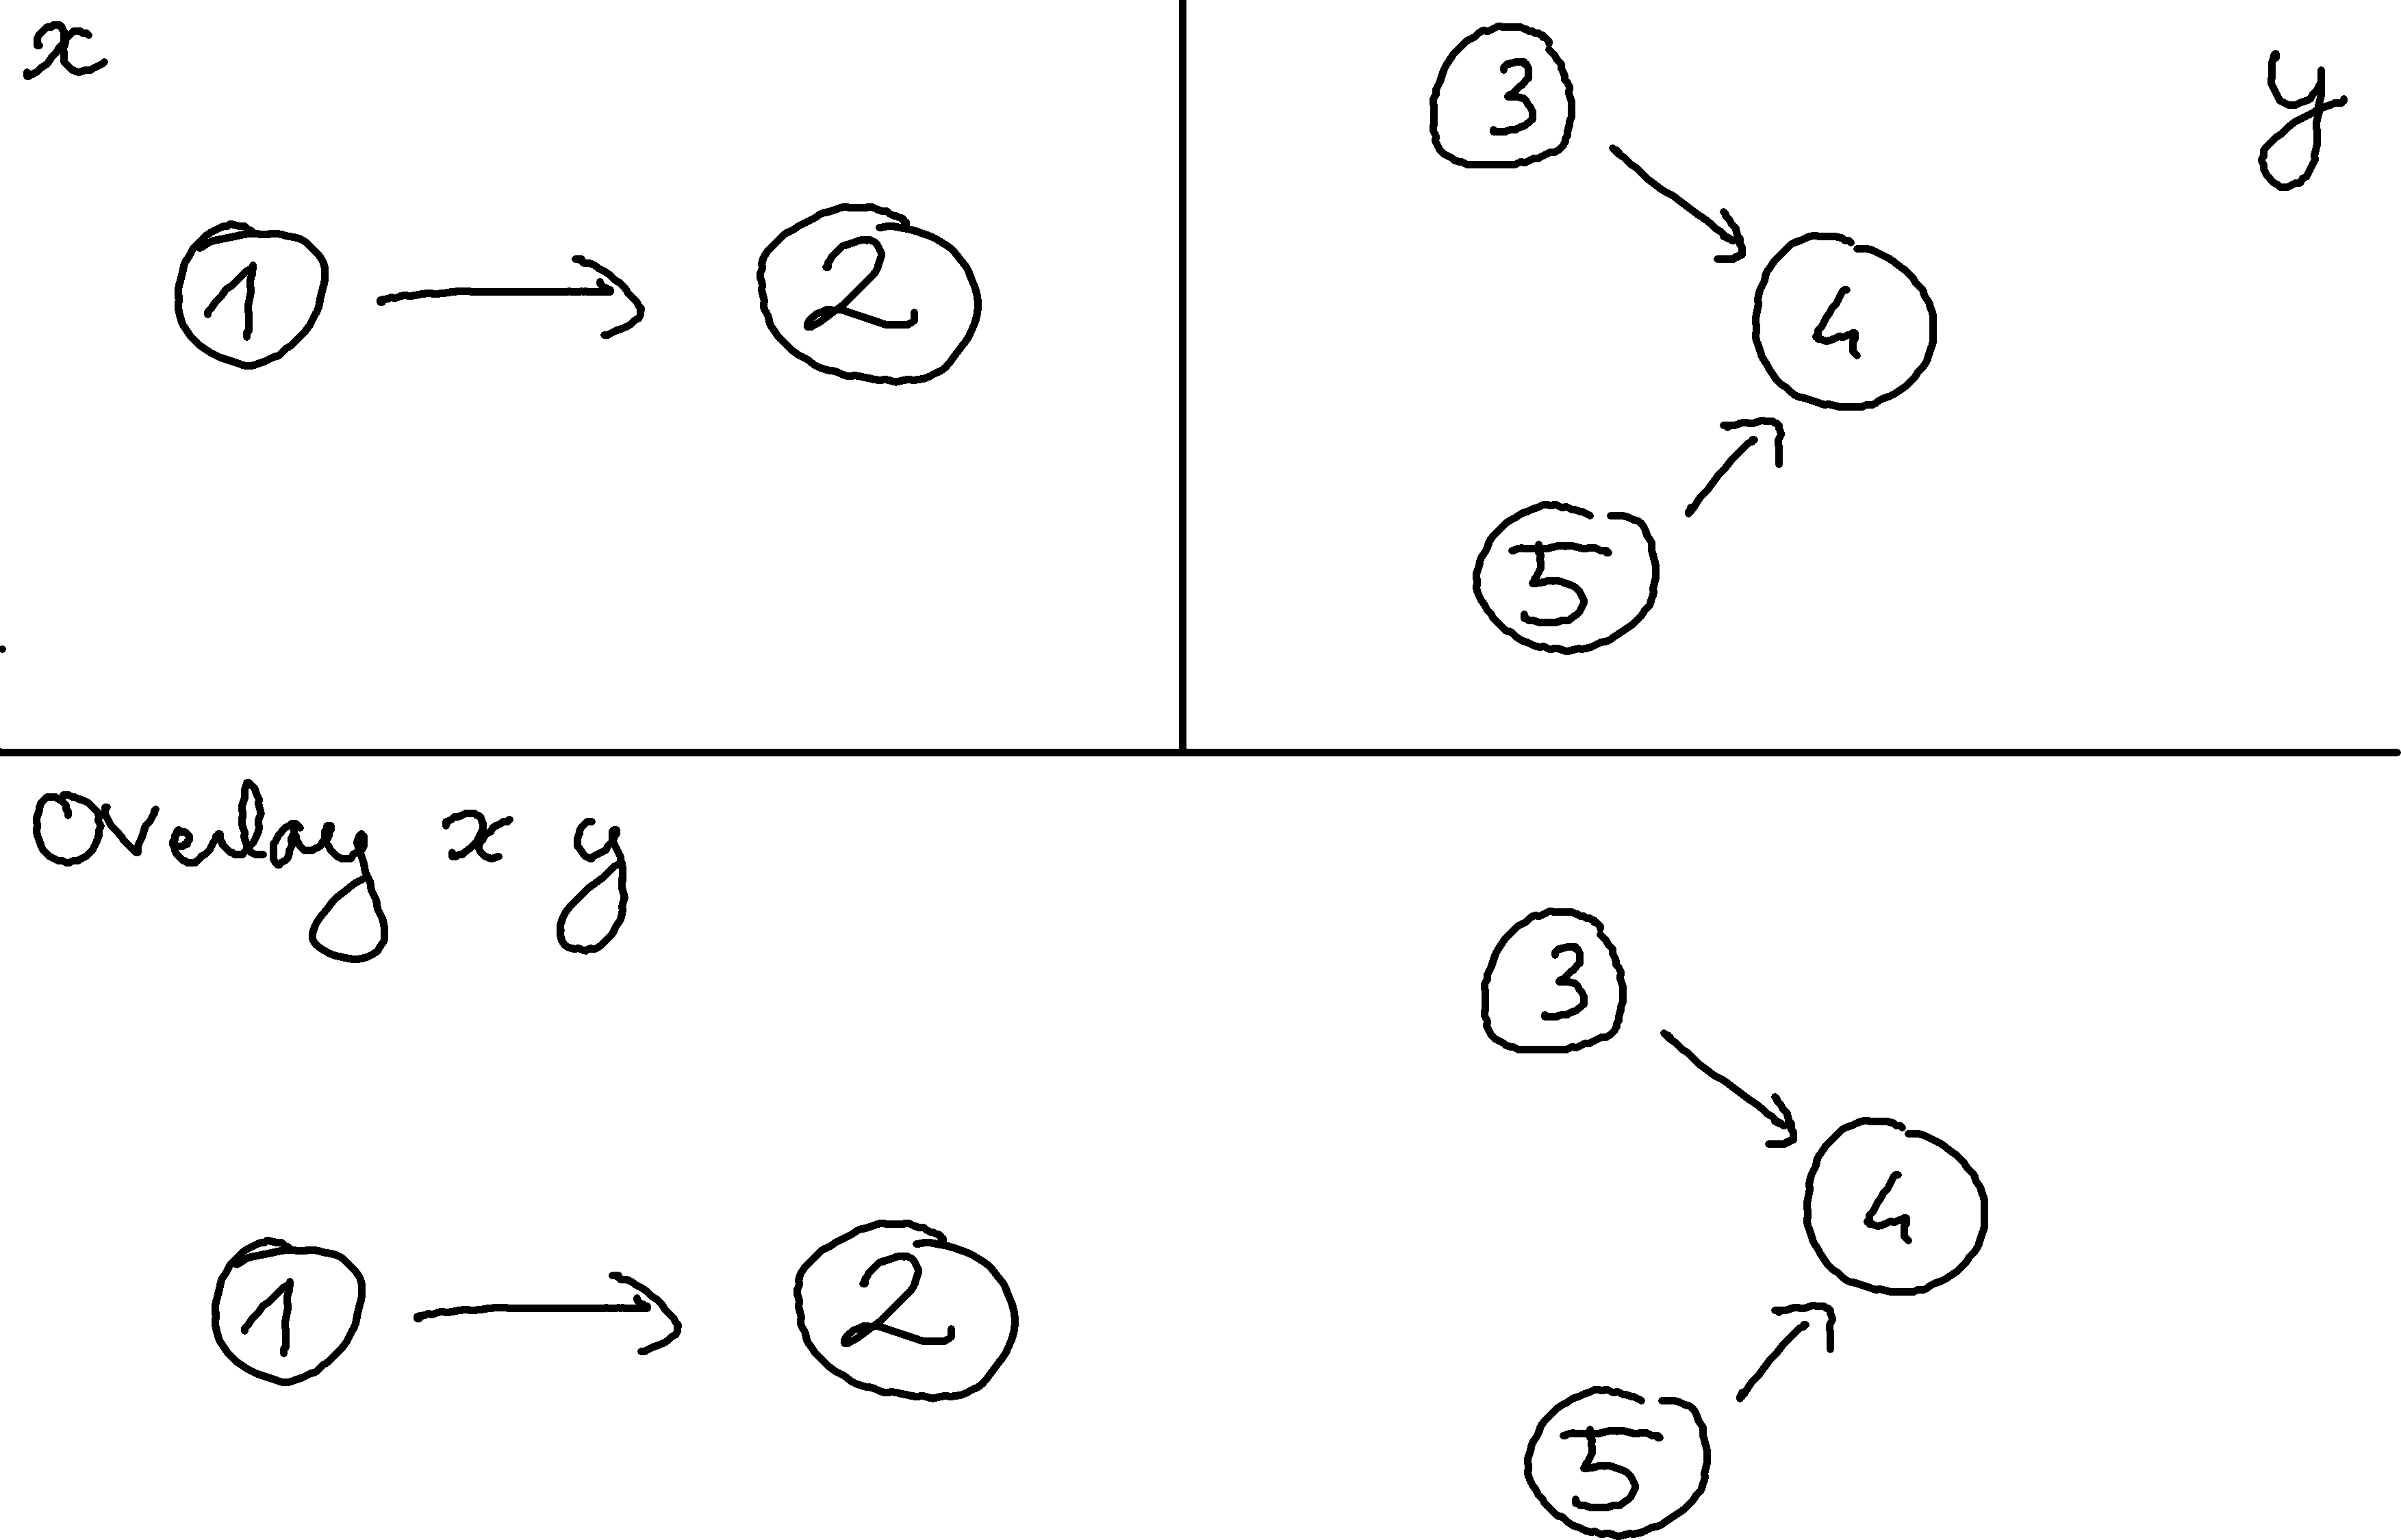
\includegraphics[scale=0.4]{figspng/overlay.png}
\end{center}

\item You can connect two graphs, that is drawing an edge from each vertex of the left side to each vertex to the right side.

\begin{center}
	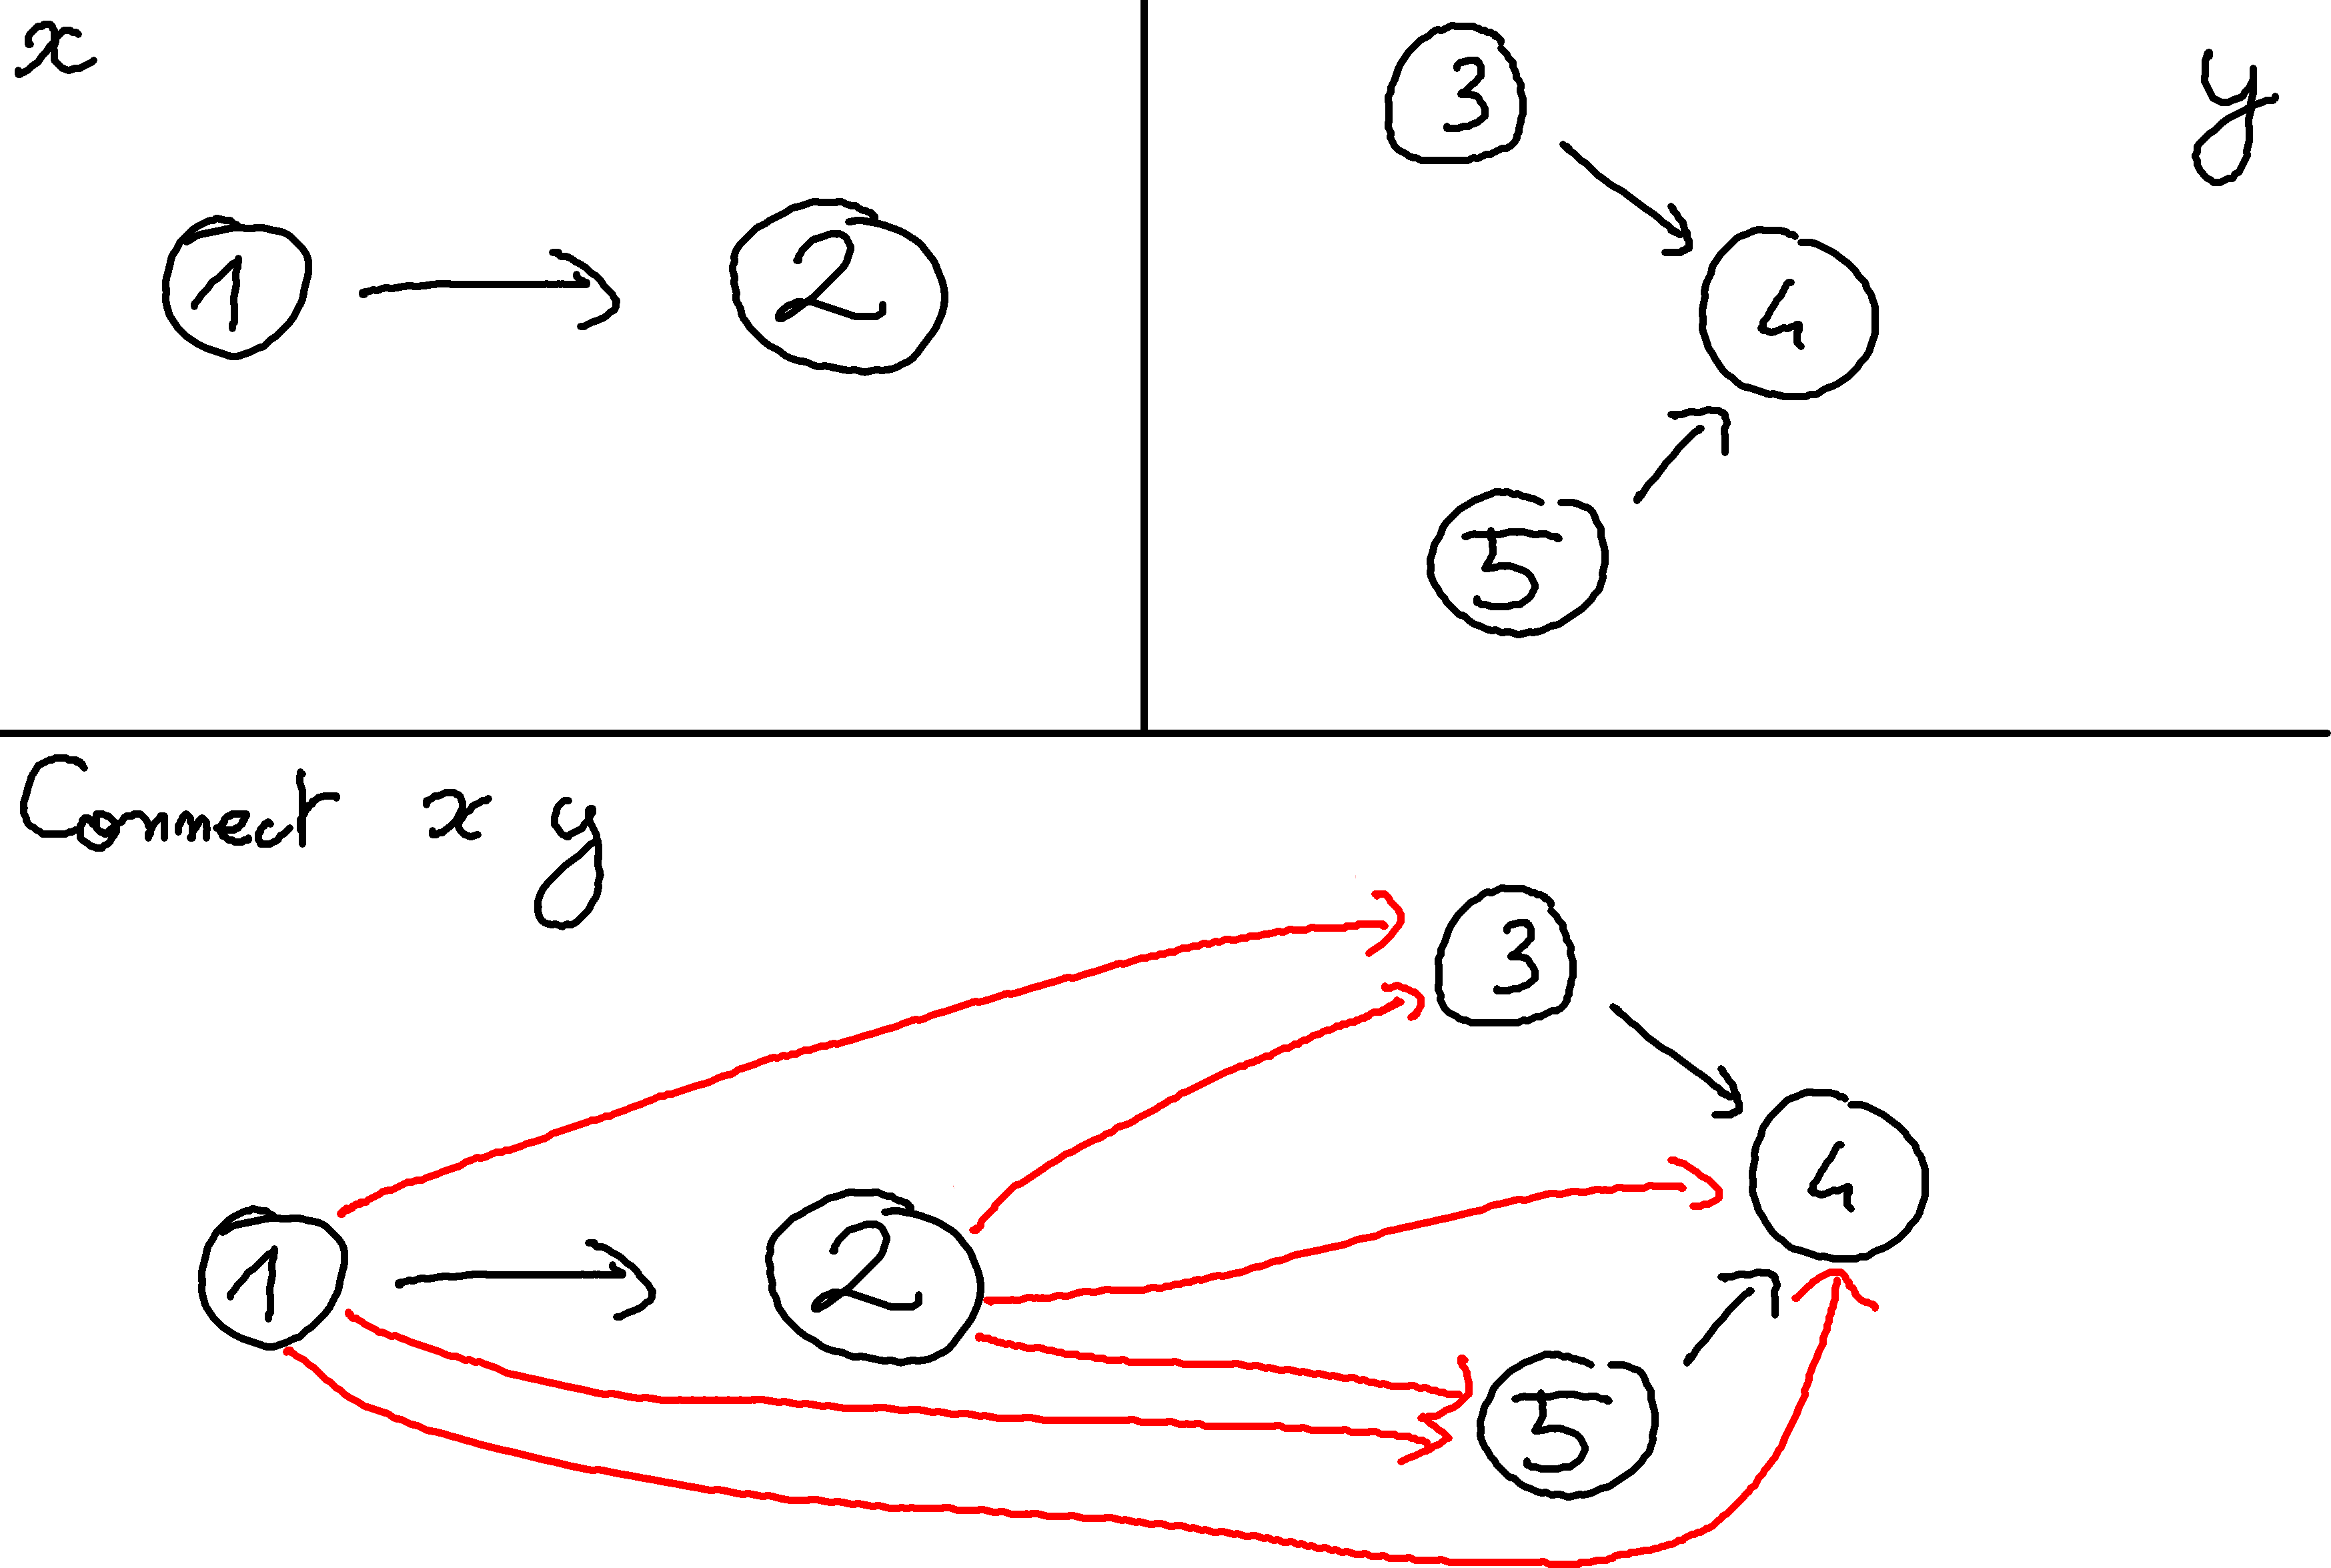
\includegraphics[scale=0.4]{figspng/connect.png}
\end{center}

\end{enumerate}

Simple, no?

\subsection{Some examples}

So, how to use this definition? Here some examples:

\begin{itemize}
	\item A single path, from a vertex 0 to a vertex 1 can be viewed as \verb|Connect (Vertex 0) (Vertex 1)| 
	\begin{center}
	
\includegraphics[scale=0.5]{figspng/e2.png}
	\end{center}
	\item A triangle, with an edge from vertex 0 to vertex 1, an edge from vertex 0 to vertex 2, and an edge from vertex 1 to vertex 2 can be viewed as  \verb|Connect (Vertex 0) (Connect (Vertex 1) (Vertex 2))| 
	\begin{center}
	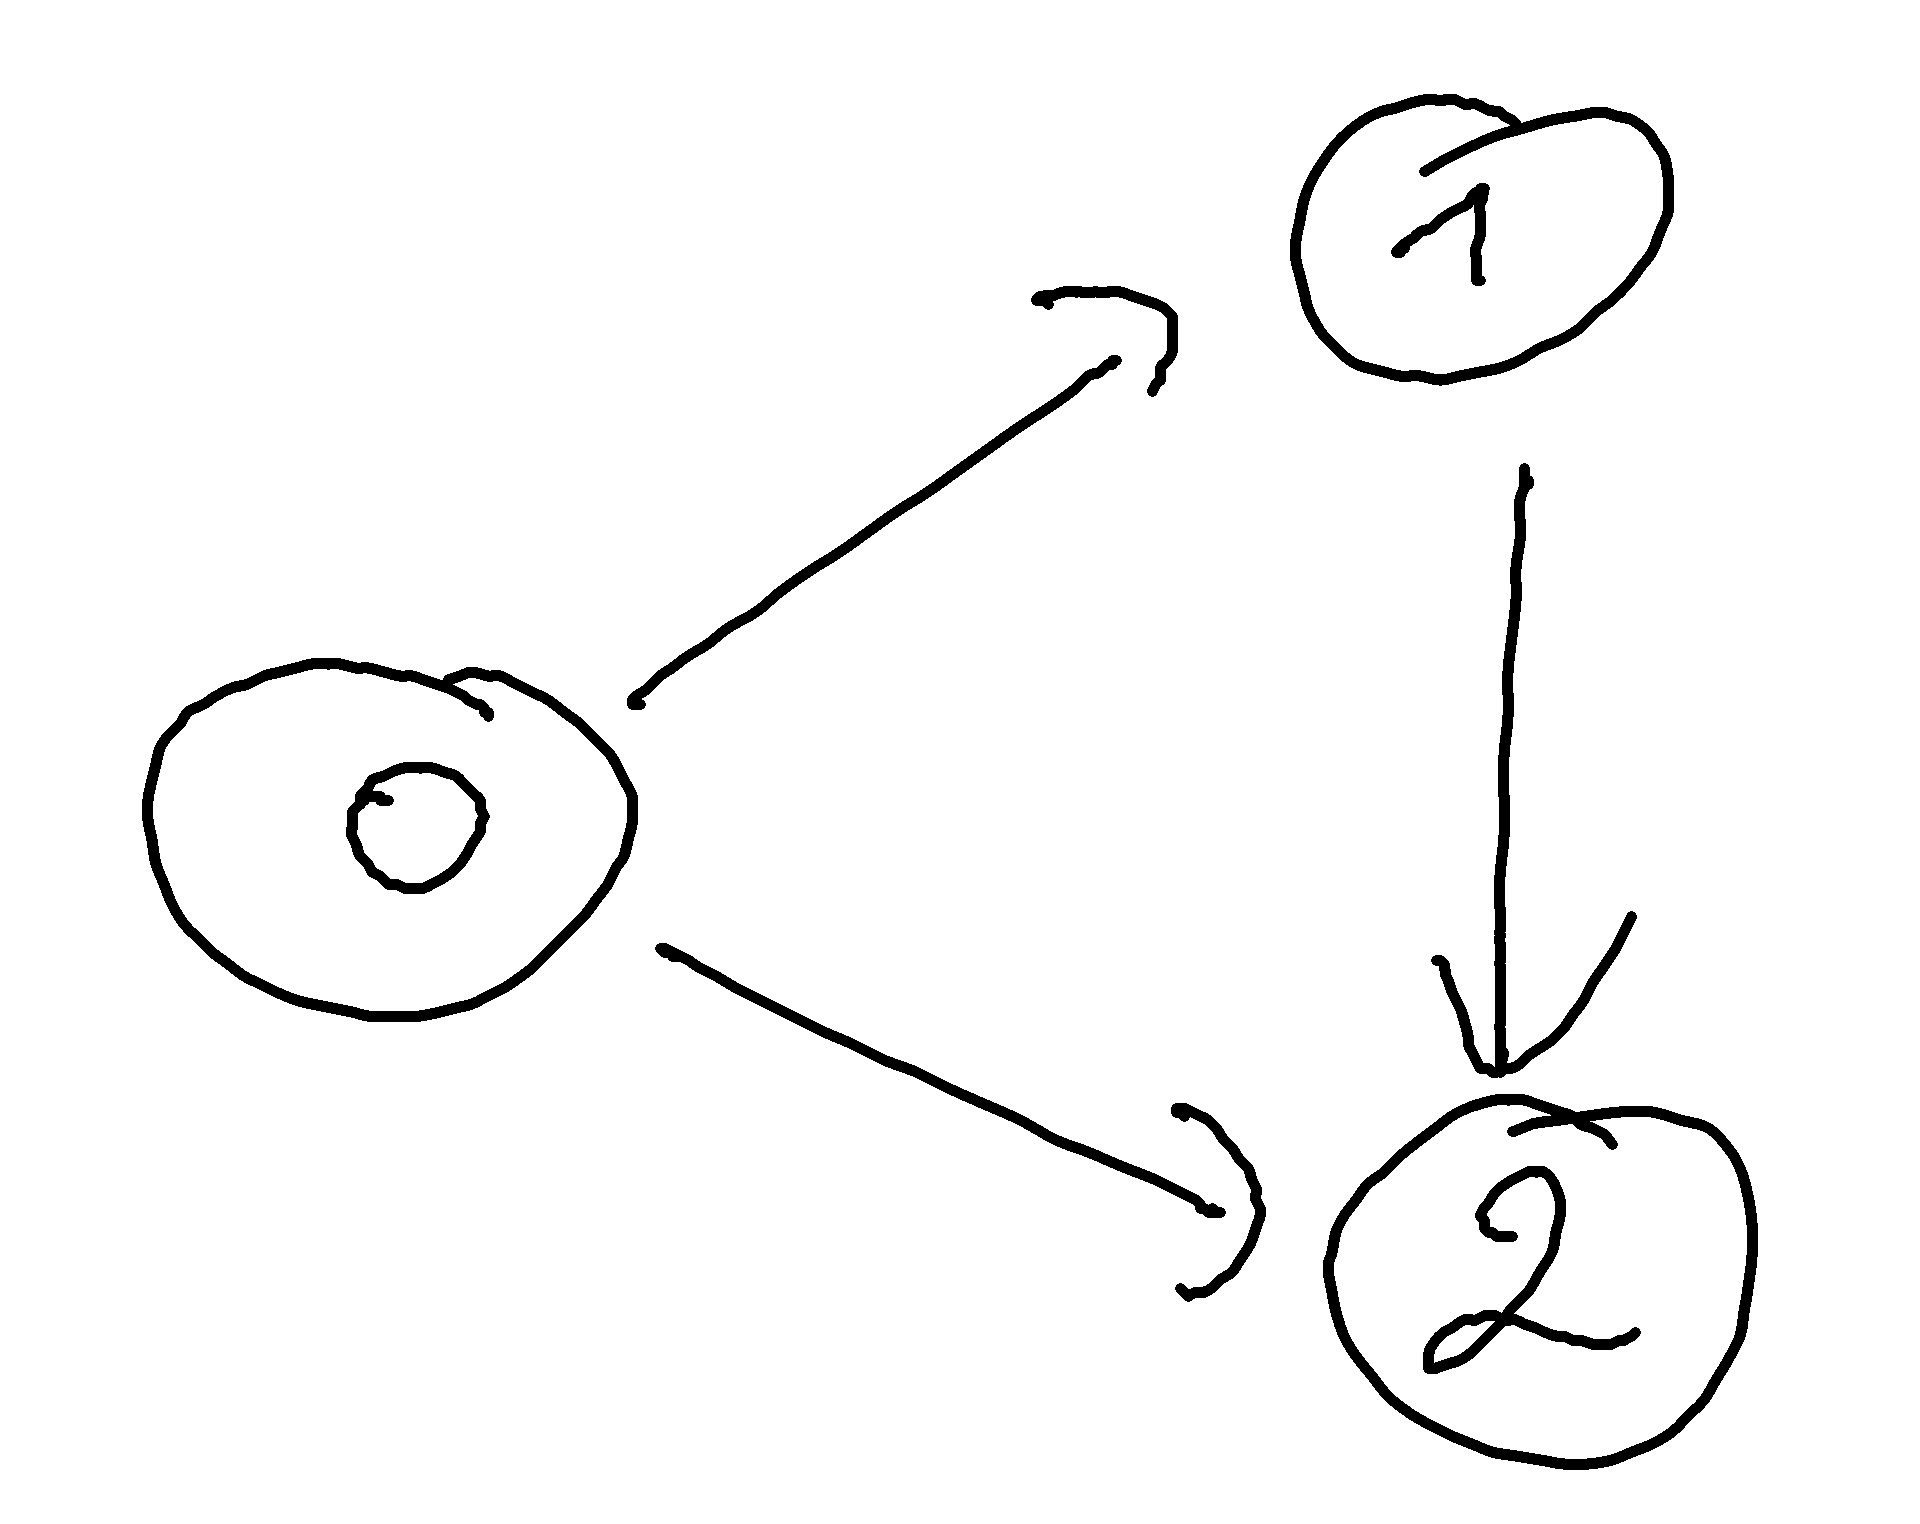
\includegraphics[scale=0.5]{figspng/e1.png}
	\end{center}

\end{itemize}

"Berk, but writing big graphs by hand can become very annoying !". Don't worry, there are some shortcuts.

\section{Going deeper in the definition}

\subsection{The Num instance}
\verb|Overlay| and \verb|Connect| looks like operators, and we want to use them as. So we pose:

\begin{lstlisting}[language=Haskell, frame=single]
(+) = Overlay
(*) = Connect
\end{lstlisting}

In fact, if we have something of the \verb|Num| instance, we can transform it directly into a graph using \verb|Vertex|. This leads to this instance:

\begin{lstlisting}[language=Haskell, frame=single]
instance Num a => Num (Graph a) where
	fromInteger = Vertex . fromInteger
	(+)         = Overlay
	(*)         = Connect
	signum      = const Empty
	abs         = id
	negate      = id
\end{lstlisting}

This means that, in a context of a \verb|Graph|, we have \verb|Vertex 1 == 1|, which is quite useful !

Do you see why alga is an implementation of an \emph{algebra} of graphs? There is a lot of maths here ! No please don't run away like you have seen a zombie in a graveyard ! Don't worry, this is not-so-difficult math.

\subsection{Overlay}

As usual, \verb|(+)| is \emph{associative} (the order in which you are choosing to overlay graphs is not important):
\begin{lstlisting}[language=Haskell, frame=single]
(1 + 2) + 3 == 1 + (2 + 3)
\end{lstlisting}

It is also \emph{commutative}:
\begin{lstlisting}[language=Haskell, frame=single]
1 + 2 == 2 + 1
\end{lstlisting}

It has \verb|Empty| as a neutral element:
\begin{lstlisting}[language=Haskell, frame=single]
1 + Empty == 1 == Empty + 1
\end{lstlisting}

It is \emph{idempotent} (overlaying a graph with itself is the same graph):
\begin{lstlisting}[language=Haskell, frame=single]
1 + 1 == 1
\end{lstlisting}

\subsection{Connect}
As usual, \verb|(*)| is \emph{associative} (the order in which you are choosing to connect graphs is not important):
\begin{lstlisting}[language=Haskell, frame=single]
(1 * 2) * 3 == 1 * (2 * 3)
\end{lstlisting}

It is NOT \emph{commutative} (drawing an edge from vertex 1 to vertex 2 is not the same as drawing an edge from vertex 2 to vertex 1):
\begin{lstlisting}[language=Haskell, frame=single]
1 * 2 /= 2 * 1
\end{lstlisting}

And it has \verb|Empty| as a neutral element:
\begin{lstlisting}[language=Haskell, frame=single]
1 * Empty == 1 == Empty * 1
\end{lstlisting}

It can absorb (connecting three times the same graph is the same as connecting two times the same graph)
\begin{lstlisting}[language=Haskell, frame=single]
1 * 1 * 1 == 1 * 1
\end{lstlisting}

\subsection{The two together}
Do you remind when you have discovered that you can mix $+$ and $*$ in the same equation ? This is the same thing here !
\begin{lstlisting}[language=Haskell, frame=single]
1 + (2 * 3) == 1 * 2 + 1 * 3
\end{lstlisting}

Whew, this is done we can  make a step forward.

\section{The benefits of the definition}
\subsection{foldg}
On of the very advantage given by this representation is the ability to define the \verb|foldg| function, a kind of adapted \verb|fold| for graph:
\begin{lstlisting}[language=Haskell, frame=single]
foldg :: b -> (a -> b) -> (b -> b -> b)
      -> (b -> b -> b) -> Graph a -> b
foldg e v o c = go
	where
	go Empty         = e
	go (Vertex  x  ) = v x
	go (Overlay x y) = o (go x) (go y)
	go (Connect x y) = c (go x) (go y)
\end{lstlisting}
In other words, the \verb|foldg| function take a base case for \verb|Empty| graphs, something to transform a \verb|Vertex|, and combining functions when we encounter \verb|Overlay| or \verb|Connect|.

\subsection{Transpose}

We have a wonderful graph and we want to \verb|transpose| it. Using \verb|foldg| this is a piece of cake:

\begin{lstlisting}[language=Haskell, frame=single]
transpose :: Graph a -> Graph a
transpose = foldg Empty Vertex Overlay (flip Connect)
\end{lstlisting}

\subsection{Induce}

Still not convinced ? Let's try to build an induced sub-graph. An induced sub-graph is a sub-graph that "forget" about some vertices and all edges to and from these vertices.

So, we are going to code the \verb|induce :: (a -> bool) -> Graph a -> Graph a| function. We will use \verb|foldg| (that the good point of tutorial, you could almost write this yourself)

What is the base case ? Do we need to change an \verb|Empty| graph ? No of course:

\begin{lstlisting}[language=Haskell, frame=single]
induce :: (a -> Bool) -> Graph a -> Graph a
induce predicate = foldg
  Empty 
  undefined
  undefined
  undefined
\end{lstlisting}

Then if we encounter a vertex, we need to verify if it satisfy the predicate. If it does not, we will simply replace it... let's say by the empty graph !

\begin{lstlisting}[language=Haskell, frame=single]
induce :: (a -> Bool) -> Graph a -> Graph a
induce predicate = foldg 
  Empty
  (\x -> if predicate x then Vertex x else Empty)
  undefined
  undefined
\end{lstlisting}
 
And finally do we need to touch connection between base graphs ? Not at all! Remember, \verb|Empty| is the neutral element of \emph{both} \verb|Connect| and \verb|Overlay|. So we can leave our empty graphs inside the structure without problem (don't worry, the real implementation get rid of these empty leaves). So we come to:

\begin{lstlisting}[language=Haskell, frame=single]
induce :: (a -> Bool) -> Graph a -> Graph a
induce predicate = foldg 
  Empty 
  (\x -> if predicate x then Vertex x else Empty)
  Overlay
  Connect
\end{lstlisting}

So simple, isn't it ?
 
\section{Useful instances}
Alga's graphs are instance of some classical class

\subsection{Functor}
Not so surprisingly, \verb|Graph| is an instance of \verb|Functor|
\begin{lstlisting}[language=Haskell, frame=single]
instance Functor (Graph a) where
  fmap _ Empty = Empty
  fmap f (Vertex a) = Vertex $ f a
  fmap f (Overlay a b) = Overlay (fmap f a) (fmap f b)
  fmap f (Connect a b) = Connect (fmap f a) (fmap f b)
\end{lstlisting}
 
This means that if you have something to transform a \verb|a| in a \verb|b| then you can transform a \verb|Graph a| into a \verb|Graph b| 
 
Alert ! Alert ! Haskeller's alarm ring ! If there is a \verb|Functor| instance, is there a \verb|Monad| one ?

\subsection{Monad}
\verb|Graph| are indeed a \verb|Monad| instance:
\begin{lstlisting}[language=Haskell, frame=single]
instance Monad (Graph a) where
  return  = Vertex
  g >>= f = foldg Empty f Connect Overlay g 
\end{lstlisting}

You can convert anything into a graph, simply by transforming it in a single vertex. Moreover, if you can produce a graph from a type \verb|a| then you can replace every vertex of a \verb|Graph a| with the result, transforming it into a \verb|Graph b|.

For example, one can redefine the previously-viewed \verb|induce| as:

\begin{lstlisting}[language=Haskell, frame=single]
induce :: (a -> Bool) -> Graph a -> Graph a
induce predicate g
  = g >>= (\x -> if predicate x then Vertex x else Empty)
\end{lstlisting}

\subsection{Foldable}
We can in fact define a \verb|Foldable| instance for \verb|Graph|. It could be:

This means that you have access to "lists-like" functions (like \verb|elem|, \verb|null|)

\end{document}